\section{Tasks schedule}

The project's life-cycle in composed by five main processes

\begin{enumerate}
	\item Requirements analysis and specifications definition
	\item Architecture design 
	\item Integration testing
	\item Project plan development
	\item Project implementation
\end{enumerate}

In the following of this section, for each of the above mentioned process the scheduling of each composing task is presented, pointing out the forecasted starting point, dead-lines and eventual task dependencies.
The scheduling activity is performed basing on the project's duration estimated during the effort and cost estimation analysis.

It's worth noting that for the first four activities the dead-lines has been already defined.

Even though the implementation tasks are perfectly ordered one after the other, during the implementation it is likely that this order will not be followed due to possible errors or changes in the system structure.

The following images show the tasks related to this project.

\begin{figure}[H]
	\centerline{
		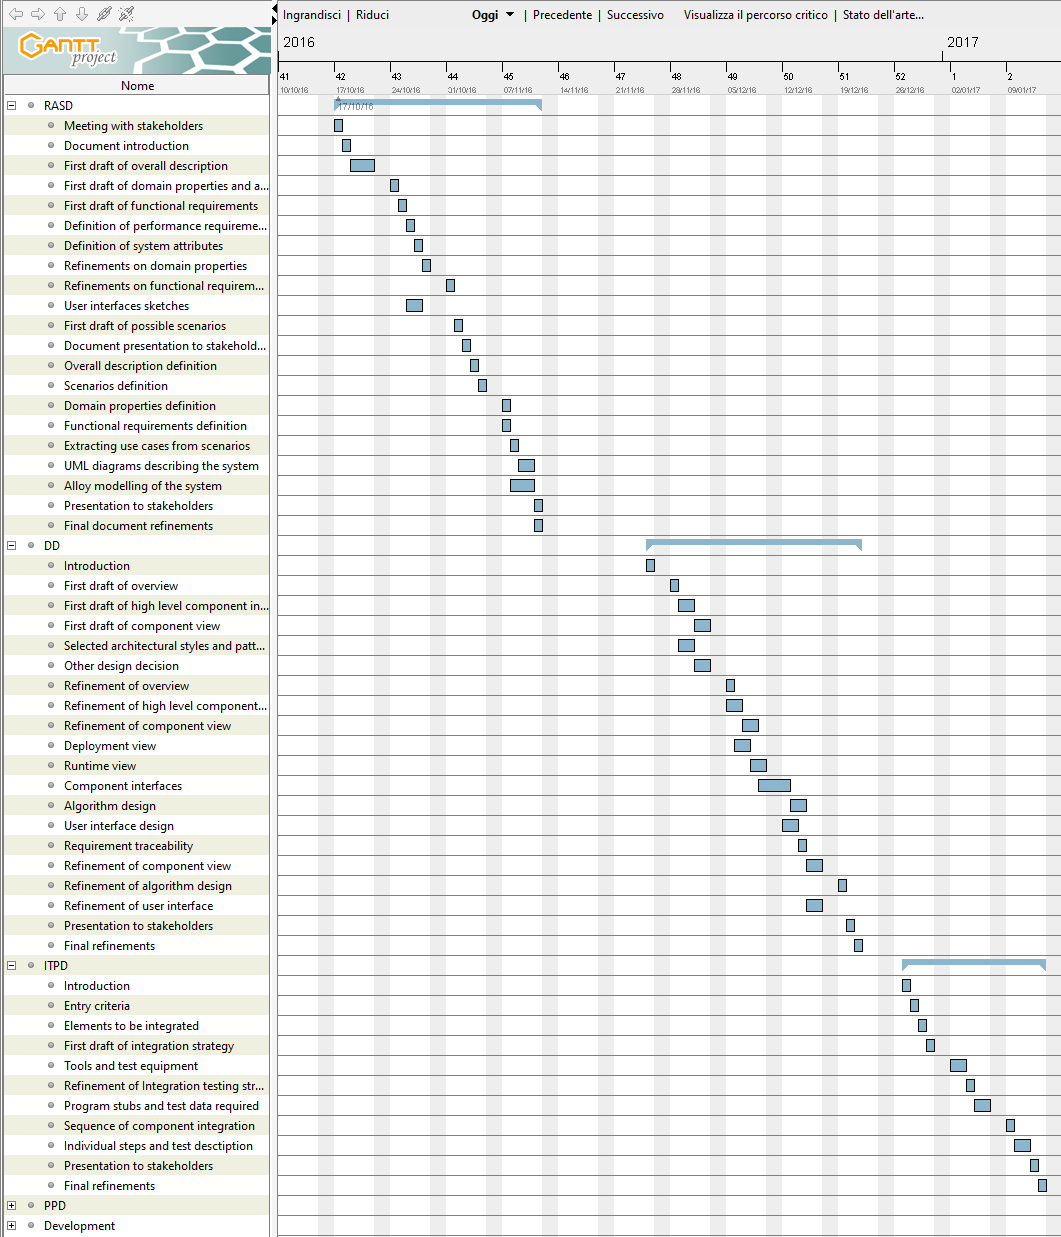
\includegraphics[width=500px]{../Datas/images/tasks-schedule-1.png}
	}
	\caption{Project tasks 1}
		\label{fig:tasks-1}
\end{figure}

\begin{figure}[H]
	\centerline{
		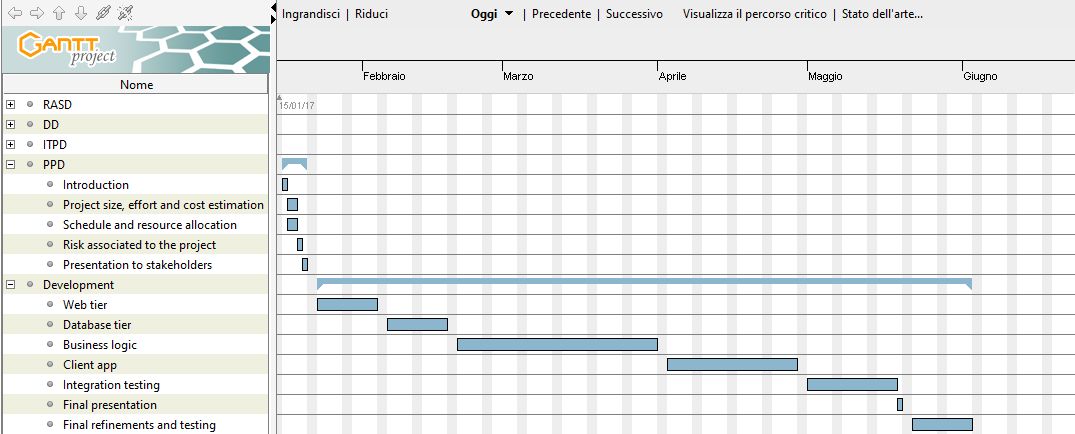
\includegraphics[width=500px]{../Datas/images/tasks-schedule-2.png}
	}
	\caption{Project tasks 2}
		\label{fig:tasks-2}
\end{figure}

\newpage

Following is a more accurate definition of each task deadline.

\begin{figure}[H]
	\centerline{
		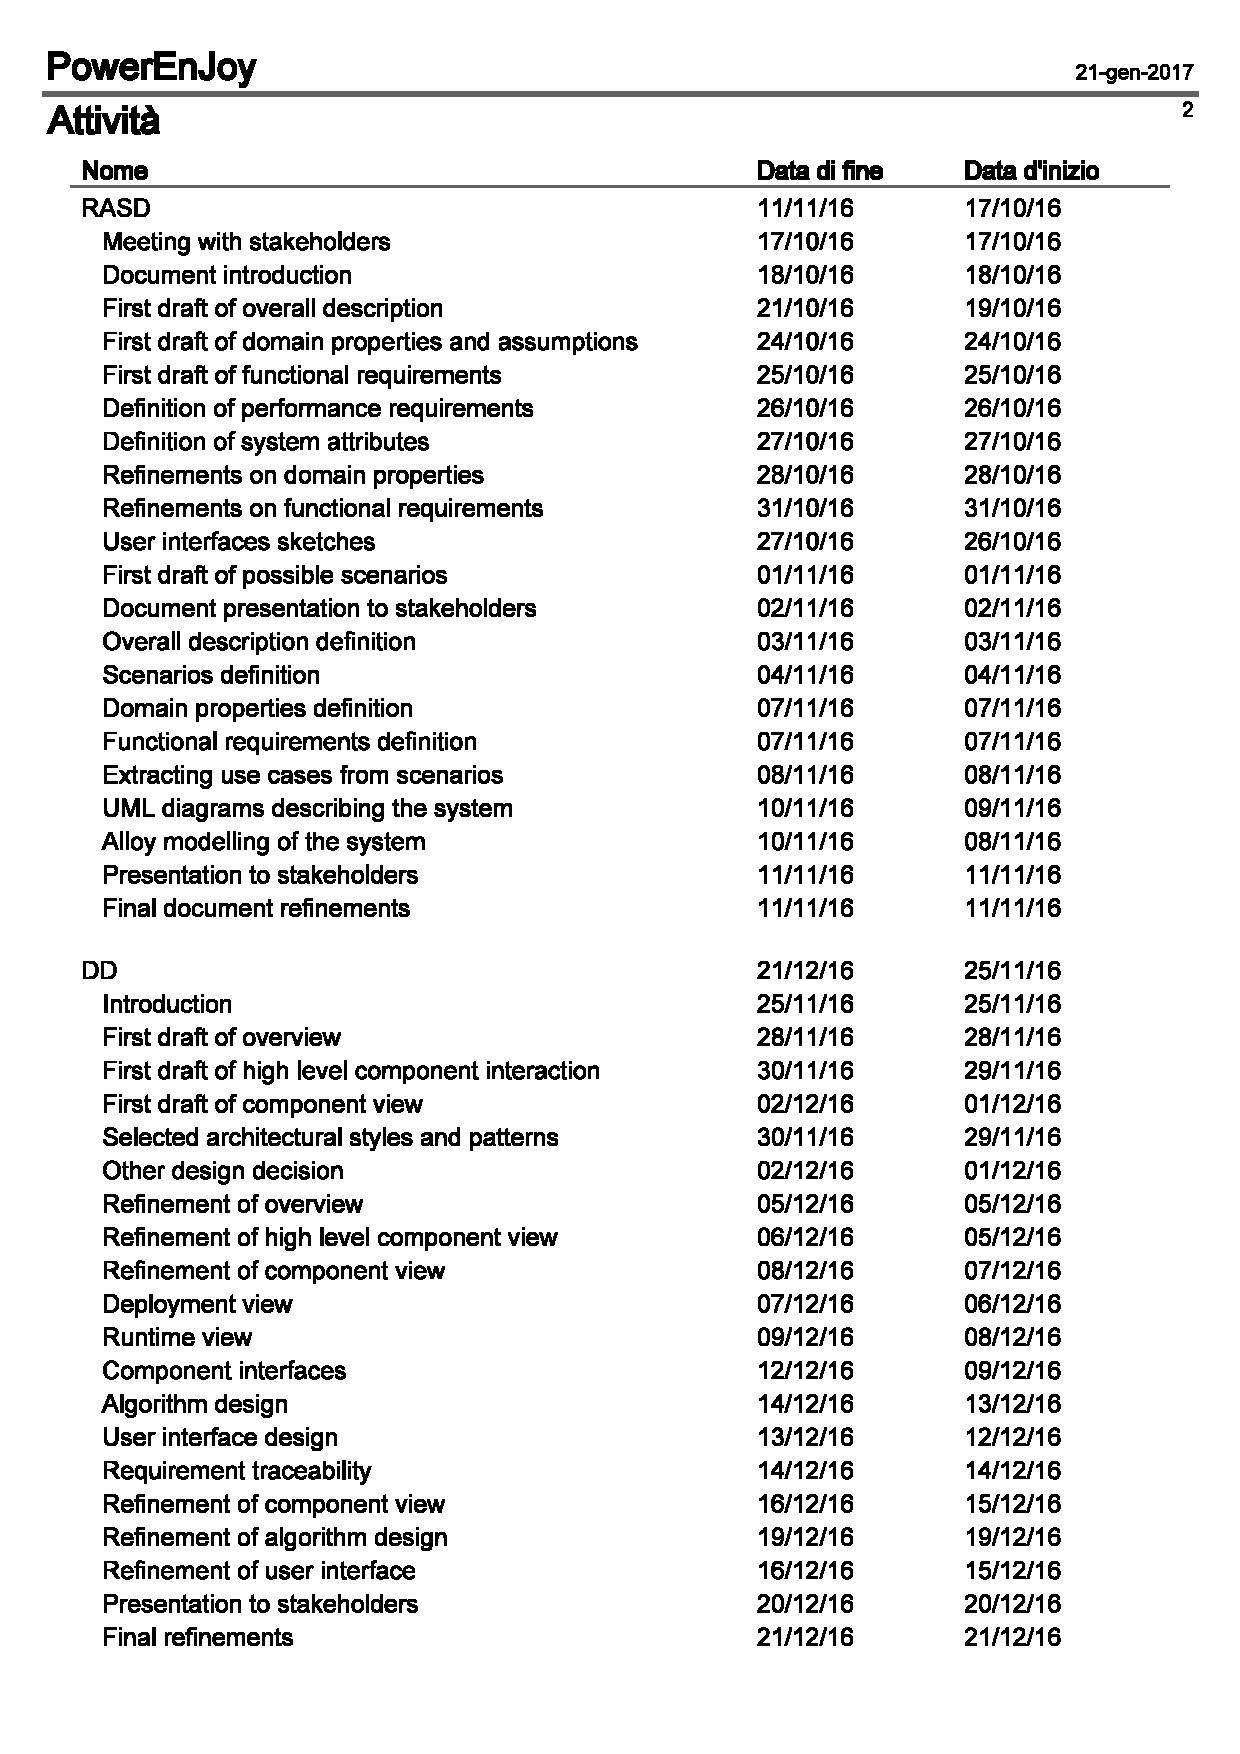
\includegraphics[width=371px]{../Datas/schedule-dates-1.pdf}
	}
		\label{fig:tasks-2}
\end{figure}

\begin{figure}[H]
	\centerline{
		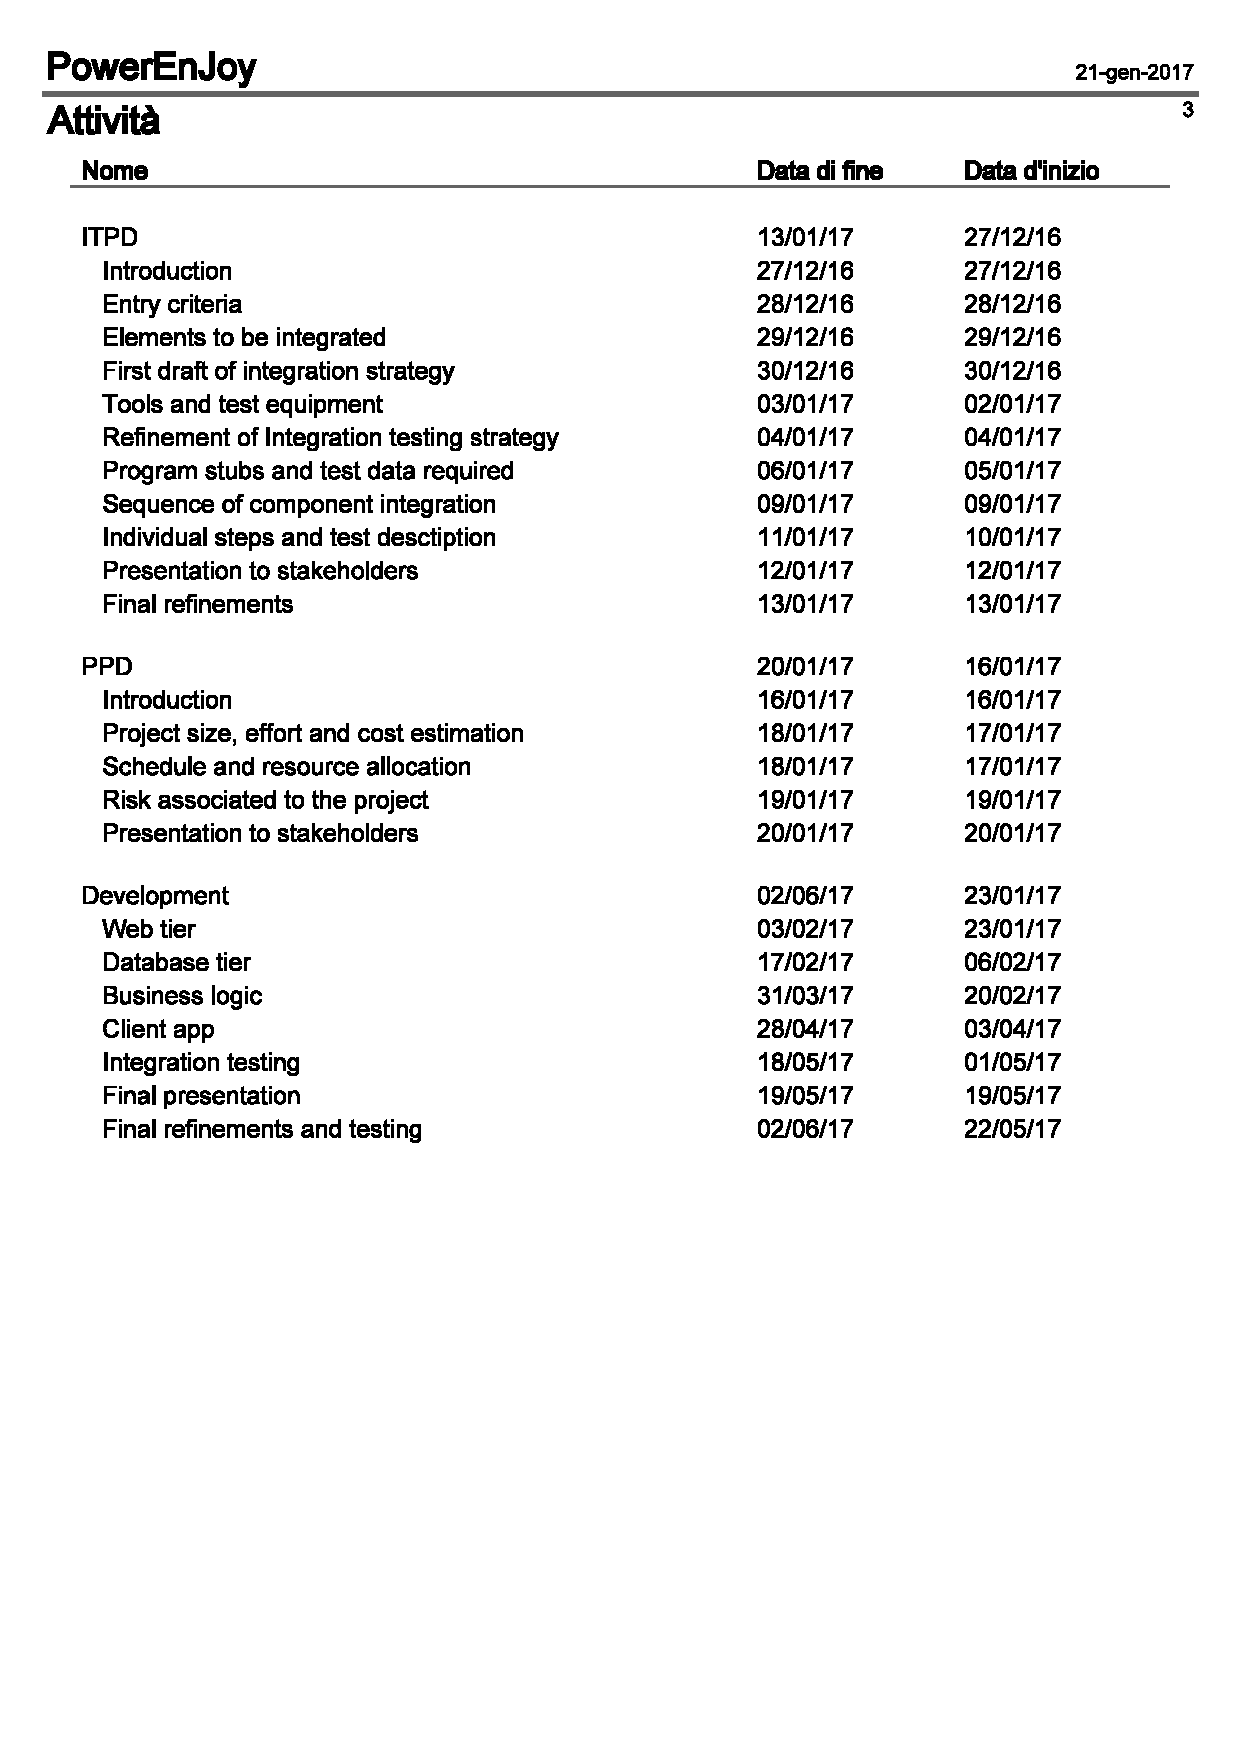
\includegraphics[width=400px]{../Datas/schedule-dates-2.pdf}
	}
		\label{fig:tasks-2}
\end{figure}
